\documentclass[12pt]{article}
\usepackage{lingmacros}
\usepackage{tree-dvips}
\usepackage[english]{babel}
\usepackage{amsthm}
\usepackage{hyperref}
\usepackage{amsmath}

\newtheorem{theorem}{Theorem}[section]
\newtheorem{lemma}[theorem]{Lemma}
\newtheorem{claim}[theorem]{claim}
\usepackage[left=1in, right=1in, top=1in, bottom=1in]{geometry}

\usepackage{amsmath}
\usepackage{amssymb}
\usepackage{tikz}
\usepackage{mathtools}
\usetikzlibrary{automata,positioning,arrows}
\usepackage[left=1in, right=1in, top=1in, bottom=1in]{geometry}
\usepackage{amsmath}
\newcommand{\N}{\mathbb{N}}
\newtheorem{prop}{Proposition}
\usepackage{tikz}
\usetikzlibrary{automata,positioning,arrows}
\usepackage{algorithm}
\usepackage{algpseudocode}
\usepackage{enumitem}
\usepackage[T1]{fontenc}
\setcounter{tocdepth}{2} % + subsubsections
\newtheorem*{claim*}{claim}

\newlength{\drop}
%COMPUTATIONAL MODELS \\ $\sim$ ALL EXERCISE SOLUTION
\begin{document}
  \begin{titlepage}
    \drop=0.1\textheight
    \centering
    \vspace*{\baselineskip}
    \rule{\textwidth}{3.6pt}\vspace*{-\baselineskip}\vspace*{6pt}
    \rule{\textwidth}{1.4pt}\\[\baselineskip]
    {\huge\textbf{COMPUTATIONAL MODELS \\ $\thicksim$ EXERCISES SOLUTION    $\thicksim$ }\\[0.3\baselineskip]{\Large TAU  SPRING 2022} }\\[0.4\baselineskip]
    \rule{\textwidth}{3.6pt}\vspace*{-\baselineskip}\vspace{6pt}
    \rule{\textwidth}{1.6pt}\\[\baselineskip]
    \scshape    
    
    \vspace*{4\baselineskip}
    Author \\[\baselineskip]
    {\Large \textbf{Saar Barak} \par}
    \vspace*{5\baselineskip}
    %\includegraphics[scale=0.2]{meme 2.png}\\
    \pagebreak
    \tableofcontents
    \par
  \end{titlepage}
  
  
\begin{center}
\section{$\sim$ Assignment 1 $\sim$}
\end{center}
\subsection{Exercise 1}
Given a Boolean function $f : \lbrace0, 1\rbrace
^n \rightarrow \lbrace0, 1\rbrace$ and a boolean circuit C of size
$|C| = s$ that computes f, Lets proof that there existences of a boolean circuit $C'$ that's stand with the question property.
\begin{claim}
Any simple logic statement that uses $\vee$ or $ \wedge$ before $ \neg$ can be re-form to $\neg$ before $\vee$ or $ \wedge$ using one additional gate
\end{claim}
\begin{proof}
using De-Morgan law for  $ x,y \in \lbrace0, 1\rbrace$ : $\neg(x \vee y)$= $ \neg x \wedge \neg y$ and on the same way for $\neg(x \wedge y)$= $ \neg x \vee \neg y$, we apply the same statement using extra one gate in total. 
\end{proof}
using the claim above we can intuitive say that we need to "roll down the tree" all the NOT gates, and from quick indication I  can claim the following.
\begin{claim}
if $P$ have some cycle $C$ size $K$ that compute it $\Rightarrow$ three is some cycle $|C'|= |2K-1|$ that can computes $P$ where all the  $\neg$ gate's before any $ \wedge$ or $\vee$ gates
\end{claim}
\begin{proof}
the indication base case is given from claim0.1, so for some Atomic  $P$ where $P_i \in \lbrace0, 1\rbrace \Rightarrow$ in total $|K|$ simple gates we get:
\[  \neg (P_1 \vee P_2 \vee \dots P_n)\Rightarrow \neg P_1 \wedge \neg P_2 \wedge \dots \neg P_n  
\]
we can notice that now we need $|K|$ NOT gates and$|K-1|$ of $\wedge$ gates, and in total $|K+K-1|$  gates.
and all the  $\neg$ gate's before any $ \wedge$ gate's. \\Now lets $P_k$ be any boolean function that stand with the induction property,for some $x,y \in \lbrace0, 1\rbrace$ lets look at: 
\[ X=\neg (P_k\vee x)= \neg P_K \wedge \neg x, Y=\neg (P_k\wedge  y)= \neg P_K \vee \neg y\]
so in any case $X,Y$ can be written in $|2k-1|$ gates of $P_k$, additional NOT gate and one $\wedge$ or $\vee$ gate, in total $|2k-1+3|=|2k+2|$ under the induction assumption we know that $P$ have some $|C|=K$ that compute it ,so $C$ including the following $
\neg , \vee$ witch is size $|K+3|$ and can compute X
\end{proof}
on the same way we proof claim 0.2 we can get the same  property for  the $\wedge$ gate, so in total for some $f$ we can find for any appearance  of $\neg$ gate  $\in C$ , and each time apply De-Morgan law. based on claim 2 this new $|C'|$ hold the property (a)(b)(c).
\subsection{Exercise 2}
For $f$ that has a circuit $C$ of size $m$ over $B_\ell$,
$C$ can be written as a binary tree with $m$ internal nodes. Each internal node is
labelled by a gate, and each leaf is labelled by a variable,
for each $v \in C$ lets $L_v: \lbrace0, 1\rbrace
^k \rightarrow \lbrace0, 1\rbrace $be the circut that accept language , according to Lupanov '58 theorem its can be expressed as language over DeMorgan basis ,using the result of exercise 2 at Recitation 1 ,we know that for such $L_v$ language there is some $C$ that can accept it when  $|C|=O(2^k)$
hence for $\forall v \in C \Rightarrow M|L_v|$ can be decided with some $C_m$ size $O(m2^\ell)$.
\subsection{Exercise 3}
$\Longrightarrow$ Lets $M$ be an DFA such as $M=(Q,\sum,\delta,q_0,F)$ and assume that $M$ accept some $w \in \sum ^*
$ i.e $\hat{\delta}_{m}  (q_0,w) \in F$. using $\hat{\delta}_{m}$ definition ,lets $k_i$ be the state such as 
\[
\ \hat{\delta}_{m} (q_0,w)=k_{n}
\]
\[
\ \hat{\delta}_{m} (q_0,w)=\delta (\hat{\delta}_{m} (q_0,w_1,w_2\dots w_n-1),w_n)\Rightarrow k_{n-1}=\hat{\delta}_{m} (q_0,w_1,w_2\dots w_n-1)
\]
follow same proses for $n-2,n-3,\dots$ so for general $k_i$ on the "back-word" path
\[
\ \hat{\delta}_{m} (q_0,w_j)=\delta (\hat{\delta}_{m} (q_0,w_1,w_2\dots w_{j-1}),w_j)\Rightarrow k_{j-1}=\hat{\delta}_{m} (q_0,w_1,w_2\dots w_{j-1})
\]
hence $\forall k_i \in Q$ , $k_n \in F$,  $k_0=q_0$ and $\delta_m (k_{i-1},w_i)=k_i$ for $1 \leq i \leq n$ \\so we can claim that the sequence $k_1,k_2,\dots k_n$ stand with the property of the second equivalent DFA definition.\\\\
$\Longleftarrow$ Lets $M$ be an DFA such as $M=(Q,\sum,\delta,q_0,F)$ and we assume that\\ $\forall q_i \in Q$ , $q_n \in F$,$w_0=q_0$ and $\delta_m (q_{i-1},w_i)=q_i$ for some $w=w_1,w_2, \dots w_n$ and $q_1,q_2, \dots q_n$
\\ with the same way decribed above 
\[
\ \delta (q_0,w_1)=q_1,\hat{\delta_m}(q_0,w_1,w_2)=\delta ( \delta (q_0,w_1),w_2)=\delta( q_1,w_2)=q_2,
\]
in general
\[
\ \hat{\delta_m}(q_0,w_1,\dots ,w_j)=\delta ( \hat{\delta_m} (q_0,w_1,\dots ,w_{j-1}),w_j)=q_j
\]
\[
\ \hat{\delta_m}(q_0,w_1,\dots ,w_n)=\delta ( \hat{\delta_m} (q_0,w_1,\dots ,w_{n-1}),w_n)=q_n \in F
\]
and we proof that both definition are equivalent
\subsection{Exercise 4}
\begin{figure}[ht] % ’ht’ tells LaTeX to place the figure ’here’ or at the top of the page
\centering % centers the figure
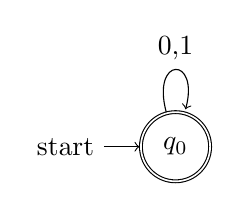
\begin{tikzpicture}
\node[state, accepting,initial]  (q1) {$q_0$};

\draw (q1) edge[loop above] node{0,1} (q1);
\end{tikzpicture}
\caption{ DFA (a) $\Sigma^*$}
\label{fig:my_label}
\end{figure}

\begin{figure}[ht] % ’ht’ tells LaTeX to place the figure ’here’ or at the top of the page
\centering % centers the figure
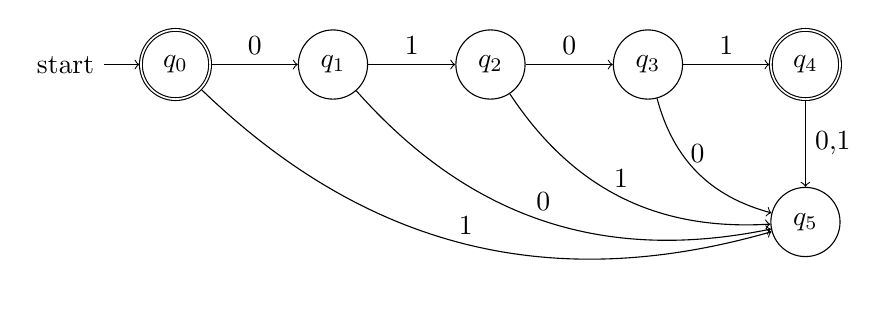
\begin{tikzpicture}
\node[state, accepting,initial]at (0, -3) (q0) {$q_0$};
\node[state, right of=q0,xshift=1cm] (q2) {$q_1$};
\node[state, right of=q2,xshift=1cm] (q3) {$q_2$};
\node[state,, right of=q3,xshift=1cm] (q4) {$q_3$};
\node[state,accepting, right of=q4,xshift=1cm] (q5) {$q_4$};
\node[state,, below of=q5,yshift=-1cm] (q6) {$q_5$};
\path[->]
(q0) edge[above] node{0} (q2)
(q2) edge[above] node{1} (q3)
(q3) edge[above] node{0} (q4)
(q4) edge[above] node{1} (q5)
(q0) edge[bend right,above] node{1} (q6)
(q2) edge[bend right,above] node{0} (q6)
(q3) edge[bend right,above] node{1} (q6)
(q4) edge[bend right,above] node{0} (q6)
(q5) edge[right] node{0,1} (q6)
;;\end{tikzpicture}
\caption{DFA (b) $\lbrace \epsilon ,0101\rbrace$}
\label{fig:my_label2}
\end{figure}

\begin{figure}[ht] % ’ht’ tells LaTeX to place the figure ’here’ or at the top of the page
\centering % centers the figure
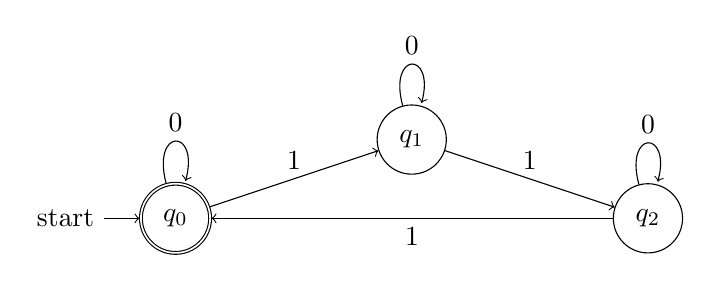
\begin{tikzpicture}
\node[state, accepting,initial]at (0, -4) (q0) {$q_0$};
\node[state, above of=q0,xshift=3cm] (q2) {$q_1$};
\node[state, right of=q0,xshift=5cm] (q3) {$q_2$};

\path[->]
(q0) edge[above] node{1} (q2)
(q2) edge[above] node{1} (q3)
(q3) edge[below] node{1} (q0)
(q0) edge[loop above] node{0} (q0)
(q2) edge[loop above] node{0} (q2)
(q3) edge[loop above] node{0} (q3)
;;\end{tikzpicture}
\caption{DFA (c) $\lbrace w| \#_1w \text{ mod 3 } \equiv 0\rbrace $ }
\label{fig:my_label2}
\end{figure}
\pagebreak
\subsection{Exercise 5}
Given n, Lets formalize the language \[L_n=\lbrace w0w_n | w \in \lbrace 0,1\rbrace^* \wedge   w_n \in \lbrace 0,1\rbrace^{n-1}
\rbrace
\]
lets present NFA $N=(Q,\Sigma,\delta,S,F)$ that accept $L_n$ , we know that any NFA can be transform to DFA .\\
\[ Q=\lbrace q_0,q_1\dots ,q_{n} \rbrace 
,\Sigma =\lbrace 0,1\rbrace
,S =\lbrace q_0\rbrace 
,F =\lbrace q_{n}\rbrace \]
\[   
\delta(q_i,\sigma) = 
     \begin{cases} 
      \lbrace q_0,q_1   \rbrace  &\quad\text{if } q_i=q_0 \wedge \sigma=0 \\
       \lbrace q_0   \rbrace  &\quad\text{if     } q_i=q_0 \wedge \sigma=1 \\
        \lbrace q_{i+1}   \rbrace  &\quad \text{if } 0<q_{i}<q_n \forall \sigma \in \Sigma \\
          \phi  &\quad\text{if } q_i=q_n  \forall \sigma \in \Sigma \\ 
     \end{cases}     
\]
\begin{claim}
N accept $L_n$
\end{claim}
\begin{proof}
$w \in L_n \Leftrightarrow$ 
\[ w \in \lbrace w0w_n | w \in \lbrace 0,1\rbrace^* \wedge   w_n \in \lbrace 0,1\rbrace^{n-1}\rbrace
\Leftrightarrow
\exists \hat{w} \in \Sigma^*.\exists \sigma \in \lbrace 0\rbrace
.w_n \in \lbrace 0,1\rbrace^{n-1}
\]
\[
\Leftrightarrow
\exists \hat{w} \in \Sigma^*.\exists \sigma \in \lbrace 0\rbrace
.\hat{\delta}_w(q_1,w_{n})\in Q
\Leftrightarrow
\exists  \hat{w} \in \Sigma^*.\exists \exists \delta(q_0,q_1) ,\hat{\delta}_w(q_1,w_{n}))\in Q
\]
\[
\Leftrightarrow
\exists  \hat{w} \in \Sigma^*.\exists  \hat{\delta}(q_0,q_n)\in Q
\Leftrightarrow
\exists \exists \dots q_i,q_j\in Q.\exists  \hat{\delta}(q_0,q_n)\in F
\]
\[
 \Leftrightarrow \delta(\hat{\delta}_w(q',q_n),\sigma)\exists q' \in Q
 \forall \sigma \in \Sigma .\hat{\delta}(q_0,q_n)\in F \Leftrightarrow
 \phi.(q_0,q_n)\in F
 \Leftrightarrow
 (q_0,q_n)\in L(N)
\]
to be honest i'm not relay sure about the last few equivalence :)
\end{proof}
Now lets show N as DFA 
\[ Q_m=\lbrace [R]|R \in Q \rbrace 
,\Sigma =\lbrace 0,1\rbrace
,\delta_0 = q_0
,F_m =\lbrace [R]|R \cap Q \neq \phi \rbrace,\delta_m([R],\sigma) =\cup_{q \in R} \delta(q,\sigma )
 \]
 \\\\
\\\textbf{Question 5 (b)}
\begin{claim}
All regular languages is closed under $\backslash$ with a
any regular language.
\end{claim}
\begin{proof}
Lets $L_1$ and $L_2$ be regular, using the regular opertor  we know already, we can immediately claim that following holds 
\[ L_1 \cap \overline{L_2} \Rightarrow L_1\backslash L_2 \text{ is regular language} 
\]
\end{proof}
\subsection{Exercise 6}
Let  $A=(Q,\sum,\delta,q_0,F)$ be a DFA, and let $w_1,w_2 \in \Sigma^*$ be words such that $\hat{\delta}(q_0, w_1) = \hat{\delta}(q_0, w_2).$
Lets proof that for every word $ w \in \Sigma^*$
it holds that $w_1w \in L(A) \Leftrightarrow w_2w \in L(A) $ 
now we set some $q_k$ such as \\$\hat{\delta}(q_0, w_1) = \hat{\delta}(q_0, w_2)=q_k \in Q$. now we construct new $A_1$ and $A_2$ in the following way:
\[ A_1=(Q,\Sigma ,\delta,q_0,q_k=F_1),
A_2=(Q,\Sigma ,\delta,q_k,F_2=F)
\]
we can notice that  $\hat{\delta}(q_0, w_1) = \hat{\delta}(q_0, w_2) \in L(A_1)$ ,and for some $w$ such as $w \in L(A_2)$ we get 
\[
w \in L(A_2) \Leftrightarrow  \hat{\delta}(q_k, w) \in F_2
 \Leftrightarrow  \hat{\delta}(q_k, w) \in F
 \]
 \[
  \Leftrightarrow  q_k \in F_1, \hat{\delta}(q_k, w)\in F  
  \]
 \[
  \Leftrightarrow \forall w'\in L(A_1).\hat{\delta} (\hat{\delta}(q_0,w')),w)\in F
   \]
 \[
    \hat{\delta} (\hat{\delta}(q_0,w_1)),w)\in F 
   \Leftrightarrow \hat{\delta} (\hat{\delta}(q_0,w_2)),w)\in F 
\]
 \[
   w_1w\in L(A)
   \Leftrightarrow    w_2w\in L(A)
\]
\\\\
\textbf{Question 6 (b)}\\
Let n be a number and let A be a DFA such that $L(A) = \lbrace0^
i1^
i
: 0 \leq
i \leq n\rbrace.
$
now follow the hint
\begin{claim}
$\hat{\delta}(q_0,0^i) \neq \hat{\delta}(q_0,0^i) $
for any $i\neq j$
\end{claim}
\begin{proof}
lets assume that $\hat{q}=\hat{\delta}(q_0,0^i) = \hat{\delta}(q_0,0^j) $ and without any loss of generality $i<j$ .from  A definition we know that $w_i:= 0^i1^i ,w_i:= 0^j1^j \in L(A)$ i.e for $\hat{\delta}(\hat{\delta}(q_0,0^j),1^i )$ we can get to for some $q\in F$. now lets look at 
 \[\hat{\delta}(q_0,w)\in F \Rightarrow\  \hat{\delta}(\hat{\delta}(q_0,0^i),1^j )=\hat{\delta}(\hat{q},1^i )
\]
under the assuming we lets look at 
\[\hat{\delta}(\hat{q},1^i )=\hat{\delta}(\hat{\delta}(q_0,0^j),1^i )=\hat{\delta}(q_0,0^j1^i)\in F
\]
and we got an contradiction.

\end{proof}
Hence the claim above hold for any $i\neq j$ and in total we find that A  has at least n accepting state.
\pagebreak
\begin{center}
\section{$\sim$ Assignment 2 $\sim$}
\end{center}
\subsection{Exercise 1}
 Define the language $L_n$ over alphabet $\sum_n = \lbrace 1, 2, ..., n\rbrace$ to be the set of words
which do not contain all the letters from $\sum_n$, now lets describe DFA $M=(Q,\sum ,\delta,q_0,F)$ s.t M accept $L_n$.
 \[
Q=\lbrace q_k | k \subseteq \lbrace \Sigma_n \rbrace \rbrace,\Sigma =\Sigma_n,q_0={q_{\phi}},F=\lbrace Q/\lbrace 1,2,3\dots n \rbrace \rbrace
\]
\[
\delta(q_k,\sigma) = 
     \begin{cases} 
      q_{k\cup \sigma } &\quad\text{if } \sigma \not\in \lbrace k \rbrace\\
       q_k &\quad\text{if     } \sigma \in \lbrace k \rbrace \\
     \end{cases}     
\]
its sufficient to see that the following claim hold to proof $M$ accept $L_n$
\begin{claim}
the DFA M \textbf{not} accept w iff $\lbrace \sigma: \sigma \in w \rbrace =\lbrace k_n \rbrace$ when $k_n$ is the set of all the letters from $\Sigma_n$
\end{claim}
\begin{proof}
First lets notice that Q contain all the subset from $\Sigma_n$ including the empty set witch correspond the empty world i.e $\lbrace \sigma \rbrace$ so in total we looking at $O(2^n)$ state for finite alphabet size $n$.\\
$\Rightarrow w\notin L_m$ if $w\in \Sigma _n^*$ since M have only one  state  lets call it $q_n$ which is not accepting state, hence $\hat{\delta}(q_0,w)=q_n$ we must go through at least n state to achieve $q_n$.  \\now using reduction on the number of district steps we done for $\hat{w}=\phi$ $\delta(q_0,\phi)=q_0$ and for some $\hat{w},\hat{\sigma}$ s.t\[ \hat{\sigma}\notin|\lbrace \sigma :\sigma \in \hat{w}\rbrace |=|k| , \hat{\delta}(q_0,\hat{w})=q_{k}\Rightarrow \delta(q_k,\hat{\sigma})=q_{k\cup \hat{\sigma}}=\hat{\delta}(q_0,(\hat{w}||\hat{\sigma})), \lbrace \sigma :\sigma \in \hat{w}||\hat{\sigma}\rbrace |=|k+1| \]
 hence we done n district steps so $| \lbrace \sigma :\sigma \in w\rbrace|=n$
 since M is DAG (except the self loops) w contain all the letters from the alphabet\\
 $\Leftarrow$ $w:= \forall \sigma \in \Sigma_n   |\sigma \in \lbrace w \rbrace $ now lets look at the first $\sigma \in w$, so $\delta(q_0,\sigma)=q_{\sigma}\in Q$ if the next letter in w hold $\hat{\sigma}\neq \sigma ,\delta(q_{\sigma},\hat{\sigma})=q_{\sigma}$ but we know that w have n district letters so in total  we get
\[
\hat{\delta}(q_0,w)=\hat{\delta}(q_{\sigma_1},\underbrace{\hat{w}}_{\lbrace \hat{w} \rbrace=\lbrace w/ \sigma_1\rbrace })=\hat{\delta}(q_{\lbrace \sigma_1,\sigma_2\dots \sigma_k \rbrace},\underbrace{\hat{w}}_{\lbrace \hat{w} \rbrace=\lbrace w/ \sigma_1,\sigma_2\dots \sigma_k \rbrace })=\delta(q_{\lbrace w/ \sigma_n \rbrace},\sigma_n)=q_n \notin F
\]  
hence $w\notin L_m$.

\end{proof}
\subsection{Exercise 2}
When A,B regular languages over same alphabet. $A \diamond B = \lbrace xy : x \in A \wedge y \in B \wedge |x| = |y|\rbrace$ lets define 
\[
\Sigma=\lbrace 0,1 \rbrace, A=L(0^*), B=L(1^*)
\]
by assuming that $ A \diamond B $ is regular language, using the property of regular language operation we get.
 \[(A \diamond B )\cap \lbrace 0^*,1^*\rbrace=\lbrace 0^i,1^i|i\geq 0 \rbrace
 \]
which lead to contradiction since $\lbrace 0^i,1^i|i\geq 0 \rbrace $ is not regular language
\subsection{Exercise 3}
$\text{\textbf{(a)} } L_1 = \lbrace w : \# a(w) \geq \# b(w)\rbrace  \text{ over } \Sigma =  \lbrace a, b, c\rbrace$\\
  $L_1$ is not regular while assuming it is. for fix $\ell$ lets $w=b^\ell a^\ell$ ,$w\in L_1$ based on Pumping Lemma we can notice $|w|>\ell$, and for any patrion of $w=xyz$ such that $|y|>0,|xy|\leq \ell$ hence y is in the form  of $b^k$ now lets look at 
  \[
  b^{\ell+k}a^{\ell}\Rightarrow \#_{b}(b^{\ell+k}a^{\ell})>\#_{a}(b^{\ell+k}a^{\ell})\Rightarrow b^{\ell+k}a^{\ell} \notin L_1
  \]
we got an contradiction hence $L_1$ is not regular\\\\
$\text{\textbf{(b)} } L_2 = \lbrace w : |w| \in \N_{even} \wedge w=w^R )\rbrace  \text{ over } \Sigma =  \lbrace 0,1 \rbrace$\\
$L_2$ is not regular while assuming it is. for fix $\ell$ lets $w=1^\ell001^\ell$ ,$w\in L_2$ based on Pumping Lemma we can notice $|w|>\ell$, and for any patrion of $w=xyz$ such that $|y|>0,|xy|\leq \ell$ hence y is in the form  of $1^k$ now lets look at
  \[
  (1^{k+\ell}001^\ell)\neq (1^{k+\ell}001^\ell)^R\Rightarrow 1^{k+\ell}001^\ell \notin L_2
  \]
we got an contradiction hence $L_2$ is not regular\\\\
$\text{\textbf{(c)} } L_3 = \lbrace w : |w| \in \N_{even} \wedge w=w^R )\rbrace  \text{ over } \Sigma =  \lbrace 0 \rbrace$\\ 
$L_3$ is regular language since we can be written  as regular expression
\[
L_3=L((00)^*)=\lbrace 00\rbrace^*=\lbrace\epsilon ,00,0000,\dots\rbrace
\]\\
$\text{\textbf{(d)} } L_4 = \lbrace w : |w| \in \N \text{ s.t } |w|=n^3 \rbrace  \text{ over } \Sigma =  \lbrace 0,1 \rbrace$\\ 
  $L_4$ is not regular while assuming it is. for fix $\ell$ lets $w=0^{\ell^3} $ ,$w\in L_4$ based on Pumping Lemma we can notice $|xyz|>\ell$, and for any patrion of $w=xyz$ such that $|y|>0,|xy|\leq \ell$. hence for some k,m such that $k+m\leq \ell$ this means that :
  \[x=0^k,y=0^m,z=0^{\ell^3-k-m}\Rightarrow,xyz=0^{\ell^3}
  \] 
by  our assumption for any $n\in \N,$ $ xy^nz=0^{\ell^3+m(n-1)}\in L_4$, lets choose n=2  \[\text{since $1\geq m \geq \ell$ we will get for some $t$}
\Rightarrow \underline{t^3=\ell^3+m }
\]
\[\text{but } t^3\geq(\ell+1)^3=\ell^3+3\ell^2+3\ell+1>
\ell^3+\ell\geq\ell^3+m\Rightarrow \underline{t^3>\ell^3+m}
\]
we got an contradiction hence $L_4$ is not regular
\subsection{Exercise 4}
\begin{claim}
For language L s.t L satisfies pumping lemma with pumping constant $\ell$
, \\$L||L$ satisfies pumping lemma with pumping constant  $2\ell$
\end{claim}
\begin{proof} Lets $w_1,w_2\in L'$ i.e $w_1\in L \wedge w_2 \in L $ and lets assume $|w_1w_2|\geq 2\ell$ to imply the pumping lemma, now we can notice that there is 2 possible scenario  
\begin{itemize}
  \item $|w_1|\geq \ell$ hence we can write $w_1$ as $w_1=xyz  \Rightarrow$ and we can write $w_1w_2$ as $w_1w_2=xyz||w_2$ which stand with the lemma property  
  \item $|w_1|<\ell$ so $|w_2|>\ell$ can write $w_2$ as $w_2=xyz$ and $|xy|\leq\ell\Rightarrow |w_1xy|\leq 2\ell,|y|>0$  we can write $w_1w_2$ as $\underbrace{w_1x}_{x'}yz$ which stand with the claim property   
\end{itemize}
\end{proof}
\subsection{Exercise 5}
\subsection*{(a)}
Lets L be a regular language over alphabet $\Sigma$. and we will proof the language $L'$ define $L'=\lbrace xyz:xy^Rz \in L \rbrace$ is regular. since L is regular $\Rightarrow$ exists some DFA that accept L $M=(Q,\Sigma ,\delta,q_0,F)$ now lets define few new DFA's  s.t:
\begin{itemize}
\item $M_{q_0,q_k}=(Q,\Sigma ,\delta,q_0,q_k)$ for any $q_k\in Q $ this DFA will cover any path that accessible from $q_0$ 
\item now lets look at $M_{q_k,q_j}=(Q,\sum ,\delta,q_k,q_j)$lets the language of $M_{q_k,q_j}$ is define by $L(M_{q_k,q_j})=\lbrace w :\exists q_k,q_j \in Q | \text{ exists path s.t }q_k \rightsquigarrow q_j \rbrace$ ,since $L(M_{q_k,q_j})$ is regular $\Rightarrow$ $rev(L(M_{q_k,q_j}))$ is regular (Recitation 3  ex.1). for any $q_k,q_j\in Q$ lets define the following language  $L(M_{q_k,q_j})^R$ 
\item $M_{q_k,F}=(Q,\Sigma ,\delta,q_k,F)$ for any $q_k\in Q $ this DFA will cover any path that end in $F$
\end{itemize}
\begin{claim}
$L'=\cup_{q_i,q_j}L(M_{q_0,q_i})||L(M_{q_i,q_j})^R||L(M_{q_j,F})$
\end{claim}
\begin{proof}
\[ w=xyz \in L' \Leftrightarrow xy^Rz \in L 
\Leftrightarrow \exists \hat{\delta}(\hat{\delta}(\hat{\delta}(q_0,x),y^R),z) \in F_m \Leftrightarrow
\]
\[
\exists M_{q_0,q_i}:\hat{\delta}(q_0,x)\in F_{ M_{q_0,q_i}} \wedge \exists L(M_{q_i,q_j})^R : y\in L(M_{q_i,q_j})^R \wedge \exists M_{q_j,F}:\hat{\delta}(q_j,z)\in F_{ M_{q_j,F}}=F_m
\]
\[ \Leftrightarrow xyz\in \cup_{q_i,q_j}L(M_{q_0,q_i})||L(M_{q_i,q_j})^R||L(M_{q_j,F})
\]
\end{proof}
\subsection*{(b)}
Lets L be a regular language over alphabet $\Sigma$. and we will proof the language $L'$ define $L'=\lbrace xy  \in \Sigma^* :(x\in L) \text{ XOR } (y\in L) \rbrace$ is regular.
using the  closure property of regular language
\begin{itemize}
\item $L=\lbrace x\in \Sigma^* : x\in L \rbrace$ and $\overline{L}=\lbrace x\in \Sigma^* : x\notin  L \rbrace$ are regular.
\item $L||\overline{L}=\lbrace xy\in \Sigma^* : x\in L \wedge y \notin L \rbrace$ and $\overline{L}||L=\lbrace xy\in \Sigma^* : x\notin L \wedge y \in L \rbrace$ are regular.
\item $(L||\overline{L}) \cup (\overline{L}||L)=\lbrace xy\in \Sigma^* : (x\in L \wedge y\notin L )\vee (x\notin L \wedge y\in L ) =(x\in L) \text{ XOR } (y\in L) \rbrace$ is regular
\end{itemize}
\subsection*{Exercise 6}
$\text{\textbf{(a)} }\lbrace w \in \Sigma^*: \#_0 (w) \leq 3 \rbrace $\\
lets express the following as regular expression 
\[
 \underbrace{1^*}_{I}\cup \underbrace{1^*01^*}_{II} \cup \underbrace{1^*01^*01^*}_{III}\cup \underbrace{1^*01^*01^*01^*}_{IV} 
\]
(I) is the regular expression of the language that contain non zeros at all.
\\ (II) is the regular expression of the language that contain exactly 1 zero.
\\ (III) is the regular expression of the language that contain exactly 2 zero.
\\ (IV) is the regular expression of the language that contain exactly 3 zero.\\
hence combine them all together will hold regular expression of the language that contain at most 3 zeros.
\\\\$\text{\textbf{(b)} }\lbrace w \in \Sigma^*:|w| \text{ mod 4}=2 \rbrace $\\
lets express the following as regular expression 
\[
 \underbrace{(0 \cup 1 )(0\cup 1) }_{(I)}\underbrace{((0\cup 1)(0\cup 1)(0\cup 1)(0\cup 1))^*}_{II}
\]
(I) is the regular expression of the language that  size is exactly 2. 
\\(II) is the regular expression of the language from size 0,4,8.. \\
hence the concatenate of (I) and (II) will hold the $|w|$ mod $4=2$ property
\pagebreak
\begin{center}
\section{$\sim$ Assignment 3  $\sim$}
\end{center}
\subsection{Exercise 1}
Considering the following language\[
\mathcal{L=} \{ \# 1^n \# x_1  \ldots x^n : \exists i\neq j \text{ s.t }
x_i \neq x_j \}
\]
Lets describe an 2-tape NTM $\mathcal{M}$ that allow the head  to stay at the same place, that recive input $\# 1^n \# (n > 1)$ and  implements the first part of decide $\mathcal{L}$
\[
Q=\lbrace q_0,q_a,q_r \rbrace,\Sigma =\{ 1,\# \},\Gamma =\{ 1,\# ,\sqcup \} 
\]
and define $\delta$ :

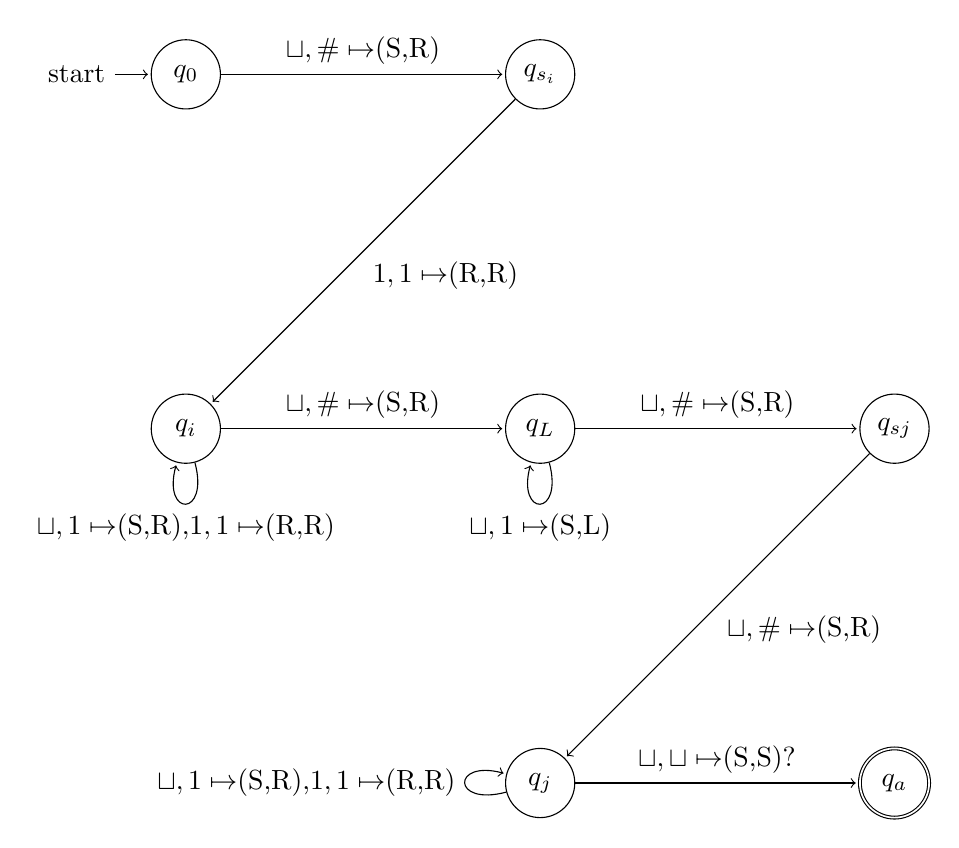
\begin{tikzpicture}[shorten >=1pt,node distance=4.5cm,on grid,auto] 
   \node[state,initial] (q_0)   {$q_0$}; 
   \node[state] (q_1) [ right=of q_0] {$q_{s_i}$}; 
   \node[state] (q_3) [below =of q_0] {$q_i$};
   \node[state] (q_4) [below  =of q_1] {$q_{L}$};     
   \node[state] (q_6) [right  =of q_4] {$q_{sj}$};        
   \node[state] (q_5) [below  =of q_4] {$q_j$};
   \node[state,accepting] (q_a) [below  =of q_6] {$q_a$};

    \path[->] 
    (q_0) edge  node {$\sqcup,\# \mapsto$(S,R)} (q_1)
    (q_1) edge node  {$1,1 \mapsto$(R,R)} (q_3)
    (q_3) edge  node {$\sqcup,\# \mapsto$(S,R)} (q_4)
    edge[loop below] node{$\sqcup,1 \mapsto$(S,R),$1,1 \mapsto$(R,R)}()
    (q_4) edge  node {$\sqcup,\# \mapsto$(S,R)} (q_6)
     edge[loop below] node{$\sqcup,1 \mapsto$(S,L)}()
    (q_6) edge  node {$\sqcup,\# \mapsto$(S,R)} (q_5)
     (q_5) edge[loop left] node{$\sqcup,1 \mapsto$(S,R),$1,1 \mapsto$(R,R)}()
     edge  node {$\sqcup,\sqcup \mapsto$(S,S)?} (q_a)
;
\end{tikzpicture}
\\The idea behind the way I generated $\delta$ is first to verify we start "legal" sequence i.e $i \neq j$ and $ i,j >0$ and split  non-deterministic for any  $i,j$ the NTM run
\pagebreak
\subsection{Exercise 2}
\subsubsection*{(a)}For DFA  $A = (Q, \Sigma, \delta, q_0, F)$. lets describe a 2-tape TM M that accept $\mathcal{L}(A)$
\[
Q=\lbrace q_{m},q_a,q_r \rbrace,\Sigma =\Sigma ,\Gamma =\Sigma \cup\{\{q\in Q\} ,\sqcup \},q_0=q_{m}
\]
\[ \delta(q,(\sigma_1,\sigma_2))=
\begin{cases} 
      (q_m,(\sigma_1,\delta(q_0,\sigma_1),(R,L)) &\quad\text{if  } \sigma_1 \in \Sigma \wedge\sigma_2=\sqcup\\
       (q_m,(\sigma_1,\delta(\sigma_1,\sigma_2)),(R,L)) &\quad\text{if } \sigma_1 \in \Sigma \wedge\sigma_2=q\in Q/F \\
       (q_a,(\sigma_1,\sigma_2),(R,L)) &\quad\text{if } \sigma_1= \sqcup \wedge\sigma_2=q\in F \\
       (q_r,(\sigma_1,\sigma_2),(R,L)) &\quad\text{if } \sigma_1= \sqcup \wedge\sigma_2=q\notin F \\
     \end{cases}  
     \]   
The idea is to save the last visted state on of A.
\subsubsection*{(b)}
For TM  $M = (Q, \Sigma, \delta, q_0, F)$. lets describe a 2-tape TM $M_2$ that accept $\mathcal{L}(M)$
\[
Q=\lbrace q_{m2},q_a,q_r \rbrace,\Sigma =\Sigma ,\Gamma =\Sigma \cup\{q\in Q\} ,q_0=q_{m2}
\]
Lets define  $\hat{q},\hat{\sigma},\hat{D}$ to be the triplet such that $\delta(q,\sigma)\longmapsto (\hat{q},\hat{\sigma},\hat{D})$
\[ \delta(q,(\sigma_1,\sigma_2))=
\begin{cases} 
      (q_m,(\hat{\sigma},\hat{q}),(\hat{D},L)) &\quad\text{if  } \sigma_1 \in \Sigma \wedge\sigma_2=\sqcup\\
       (q_m,(\hat{\sigma},\hat{q}),(\hat{D},L)) &\quad\text{if } \sigma_1 \in \Sigma \wedge\sigma_2=q\in Q \\
       (q_a,(\sigma_1,q_a),(R,L)) &\quad\text{if }  \sigma_2=q_a \wedge \forall \sigma_1 \\
       (q_r,(\sigma_1,q_r),(R,L)) &\quad\text{if }\sigma_2=q_r \wedge \forall \sigma_1 \\ \end{cases}  
     \]  The idea is kind of same as above but now we track the direction of the head of M 
     \pagebreak
\subsection{Exercise 3}
\begin{prop} Disprove $\mathcal{RE}$ is not closed under complement.\end{prop}
For $L,\overline{L}$, if both are semi-decidable $\Rightarrow$ both are decidable, (can just flip the nation reject accept)
$\Rightarrow$ if we assume $\mathcal{RE}$ closed under complement, $\forall L \in \mathcal{RE}, \overline{L} \in \mathcal{RE}\Rightarrow$ we get that $\mathcal{RE}=\mathcal{R} \Rightarrow \clubsuit $

\hrulefill
\begin{prop}  $co\mathcal{RE}$ is closed under intersection.\end{prop}
By detention $L \in co\mathcal{RE}$ if $\overline{L} \in \mathcal{RE}$. using the fact that $\mathcal{RE}$ Closures under union we can apply De-Morgan law  for some $\overline{ L_1},\overline{ L_2}\in co\mathcal{RE} $ which lead us to :  \[ L_1,L_2\in \mathcal{RE} \Rightarrow L_1\cup L_2\in \mathcal{RE}\Rightarrow \overline{ L_1\cup L_2}\in co\mathcal{RE}\Rightarrow \overline{ L_1} \cap \overline{ L_2}\in co\mathcal{RE}\]\hrulefill
\begin{prop}  $\mathcal{R}$ is closed under Kleene star.\end{prop}
w.l.o.g $\mathcal{L} \in \mathcal{R}$ such that exist TM $T$ that decide $\mathcal{L}$.now we can build an TM $M^*$ that accept $L^*$ for input x .
\begin{list}{•}{}
\item if $x=\epsilon$ Accept.
\item  partition $|x|=n$ to any combination possible ways lets say $x_{power}:=( \{x_1\},\{x_2\}\dots \{x_{2^{n-1}}\} )$
\item run $L$ for any $\forall w\in \{ x_i \} $, if for some $x_i$ L accept \textbf{all} $w\in \{ x_i\}$
Accept.
\item else Reject.
\end{list}
\hrulefill
\begin{prop}  $\mathcal{RE}$ is closed under Prefix, but $\mathcal{R}$ is not closed under Prefix,\end{prop}
\textbf{i. }Since $\mathcal{L} \in \mathcal{RE}$, there exists an enumerator $f_{\mathcal{L}}$.  Its will be sufficient to describe $f_{prefix}$ to proof that $\mathcal{L}\in \mathcal{RE}\Rightarrow \text{Prefix(}\mathcal{L})\in \mathcal{RE} $  Now lets built new $f_{prefix}$.
\[f_{prefix}=
    w:=\{ \sigma_1\dots\sigma_k \}  \forall k: 0<k<|w| \text{ for any  }f_{\mathcal{L}}=w
\] 
the idea is to use $f_{\mathcal{L}}$ output and apply Prefix on any world to create $f_{prefix}$\\\\
\textbf{ii. }Lets assume $\mathcal{R}$ closed under Prefix. and lets look at my favourite TM $M_F$  for $L_{f} \in \mathcal{RE/R}$. now lets construct new $\hat{L}$ consisting of strings from the encode of  $M_F$ and $\#$ i.e $M_F\#$
now I claim that $\hat{L}$ Accept only when its see $\#$ ,otherwise its Reject. hence exist some deterministic TM that Reject/Accept. $\hat{L}\in \mathcal{R}$, but Prefix($\hat{L})=L_f\notin \mathcal{R}\Rightarrow \clubsuit$
\subsection{Exercise 4}
Define $\text{Size}(O(n))$: \[
\text{Size}(O(n)) = \left\lbrace
\mathcal{L} :\exists \mathcal{C}:=\{C_n\}_{n\in N}\text{
s.t } \mathcal{L(C)=L} \wedge |C_n|\in O(n)  \forall n\in N
\right\rbrace
\]
\textbf{i. } Lets look at the unary language 
$\mathcal{L} \subseteq \{1^n: n \in N \}$, its immediate  that $\mathcal{L}\in\text{Size}(O(n)) $ since its needs to have a single “hardwired”
bit for indicating $1^n$. now lets look at the language $\mathcal{L_U}$
\[ \mathcal{L_U} := \{1^
n | \text{ The Turing machine encode to n halts on $\epsilon$.}\}
\]
Hence its immediate from Rice’s Theorem, or the fact that $
H_{TM\epsilon}$ $\leq_m \mathcal{L_U}$
that $\mathcal{L_U} \notin \mathcal{R}$ and $\mathcal{L_U}\in\text{Size}(O(n)) $
\\\\\textbf{ii. } We can look at some recursively   define $\mathcal{L}\in \mathcal{R}$ for example: \[
\mathcal{L} =\{1^{2^n} : n\geq0 \}
\] Since we will need circuit for each possible input length, we  may need exponential size circuit (in terms of n) to accept words in the  language.  and the following holds that $\mathcal{L} \notin \text{Size}(O(n)) $
\subsection{Exercise 5}
\begin{enumerate}[label=(\Alph*)]
\item \textbf{Prove:} If $\mathcal{L}_1 \leq_m \mathcal{L}_2$ and $\mathcal{L}_2 \leq_m \mathcal{L}_3, $ then $ \mathcal{L}_1 \leq_m \mathcal{L}_3.
$ \\\ Define $f_{1\rightarrow 2},f_{2\rightarrow 3}$ to be a computable mapping redaction  functions. now lets $w\in \mathcal{L}_1$, and by dentition  we get :
\[
w\in \mathcal{L}_1\Leftrightarrow f_{1\rightarrow 2}(w)\in \mathcal{L}_2
\Leftrightarrow f_{2\rightarrow 3}(f_{1\rightarrow 2}(w))\in \mathcal{L}_3
\]






\item \textbf{Disprove:} If $\mathcal{L}_1 \leq_m \mathcal{L}_2$ and $\mathcal{L}_2 \leq_m \mathcal{L}_1, $ then $ \mathcal{L}_1 = \mathcal{L}_2.$\\
for $H_{TM},A_{TM}$ we know that $H_{TM}\leq_m A_{TM}$ and $A_{TM}\leq_m H_{TM}$ but $A_{TM}\neq H_{TM}\Rightarrow\clubsuit$
\item \textbf{Disprove:} If $\mathcal{L}_1 \subseteq \mathcal{L}_2$  then $ \mathcal{L}_1 \leq_m \mathcal{L}_2.$\\\ Lets look at $\mathcal{L} = \Sigma^*$,$\mathcal{L} \in \mathcal{R}$ since any other $\mathcal{L}'\subseteq \mathcal{L}$. if we assume that    $\forall \mathcal{L}' \leq_m \mathcal{L}$ its will lead to  $\forall \mathcal{L} ' \in \mathcal{RE} \Rightarrow\clubsuit$
\item \textbf{Disprove:} For every  $\mathcal{L}_1,\mathcal{L}_2$, then $\mathcal{L}_1 \leq_m \mathcal{L}_2$ or $\mathcal{L}_2 \leq_m \mathcal{L}_1$\\
Lets look at $A_{TM},\overline{A_{TM}}$. If we assume $\overline{A_{TM}} \leq_m A_{TM}$ Since $\overline{A_{TM}}\notin \mathcal{RE}$
its will lead to $A_{TM}\in \mathcal{R}\Rightarrow\clubsuit$,\\ and if $A_{TM} \leq_m \overline{A_{TM}} $ Since $A_{TM}\notin \text{co-}\mathcal{RE}\Rightarrow \overline{A_{TM}}\in \mathcal{R}\Rightarrow\clubsuit$
\item \textbf{Prove:} If $\mathcal{L}$ is regular, then $\mathcal{L} \leq_m HALT$
\\Lets A  be an DFA s.t $L(A)=\mathcal{L}$ when $\mathcal{L}$ is regular. based on 2(a) we define some TM M that accept $L(A)$ and Let $M_{loop}$ be TM that loop forever for any input. hence we can define computable f :
\[f(w)=\begin{cases} 
      \langle M,w\rangle &\quad\text{if  } w\in M \\
      \langle M_{loop},w\rangle &\quad\text{if  } w\notin M\\
     \end{cases} 
\]
Which imply  $\mathcal{L} \leq_m HALT$
\end{enumerate}
\subsection{Exercise 6}
\begin{center}
\textbf{(a)} $\mathcal{L} = \{\langle M\rangle : M $ is a TM and $|L(M)| > 10\} \in  \mathcal{RE/R}$
\end{center} 

Lets describe algorithm $A_{10}$ that accept $\mathcal{L}$
\begin{algorithm}
\caption{  $A_{10}$ on input $\langle M\rangle$ }\label{alg:cap}
\begin{algorithmic}
\Require $\langle M\rangle$ is a valid encode of TM\\ else \textbf{Reject} 
\State $k$ $\leftarrow$ 1
\While {$k < \infty$} 
\State counter $\leftarrow$ 0
\For {$i$  $\leftarrow$ 1 \textbf{to } $k$ }
\State  simulate $M$ on $w_i$
for $k$ steps\Comment{$w_i$ generated from $\Sigma$ of $M$}
\If {$M$ accept}\State counter + 1
\EndIf
\EndFor
\If { counter $>10$} \textbf{Accept}
\EndIf
\EndWhile
\end{algorithmic}
\end{algorithm}
\\Its implement that we cover any optional input on $M$ and while discovered more then 10 worlds in $\mathcal{L}$ we accept. hence $\mathcal{L} \in \mathcal{RE}$
\\Now  lets proof $\mathcal{L}\notin \mathcal{R}$ using reduction from HALT$\leq_m \mathcal{L}$. now lets define $\mathcal{M}$ 
\begin{algorithm}
\caption{ $\mathcal{M}$ on input $\langle M,\hat{w}\rangle$ .}\label{alg:cap}
\begin{algorithmic}
\Require $\langle M,\hat{w}\rangle$ is a valid encode of TM and word\\ else \textbf{Reject} 
\State Ignore $\hat{w}$
\State \textbf{Write} $M$ and $w$ on the tape
\State run $M$ on $w$ \textbf{Accept} if $M$ halt
\\ else \textbf{Reject}
\end{algorithmic}
\end{algorithm}
\\I claim that exists maping function from $H_{TM}$ to $\mathcal{L}$   s.t:
\begin{list}{•}{}
\item If $\langle M,\hat{w}\rangle \in H_{TM} \Rightarrow M(\hat{w})$ halt $\Rightarrow\mathcal{M}$ accept any input $ \Rightarrow  |L(\mathcal{M})|>10\Rightarrow \mathcal{M}\in \mathcal{L} $
\item If $\langle M,\hat{w}\rangle \notin H_{TM} \Rightarrow M(\hat{w})$ not halt $\Rightarrow\mathcal{M}$ dont  accept any input $ \Rightarrow  |L(\mathcal{M})|<10\Rightarrow \mathcal{M}\notin \mathcal{L} $
\end{list}
\[
f(\langle M,w\rangle)=\begin{cases} 
     \langle \mathcal{M} \rangle  &\quad\text{if  }\langle M,w\rangle \text{ is valid input  of TM and word} \\
    \langle \mathcal{M}_{favourite} \rangle  &\quad\text{otherwise  } \end{cases} 
\]
Where  $\mathcal{M}_{favourite}$ is my favourite TM that hold $|L(\mathcal{M}_{favourite})|=10$
\\\hrulefill
     \pagebreak
\[ \text{\textbf{(B) }}\mathcal{L} = \{ M : \langle M\rangle \text{ is a TM that accepts 1 but does not accept 0}\} \in \overline{\mathcal{RE}\cup\text{co-} \mathcal{RE}}
\]
Lets look at \[ \mathcal{L}_{1\wedge\neg 2}=\{ \langle M_1,w_1,M_2,w_2\rangle | w_1 \in L(M_1) \wedge w_2 \notin L(M_2)\} \]
since we know that $\mathcal{L}_{1\wedge\neg 2}\in \overline{\mathcal{RE}\cup\text{co-}\mathcal{RE}}$ we can can apply mapping reduction. Now lets construct a TM $\mathcal{M}_{1\wedge\neg 2}$ that work as follow:
\begin{algorithm}
\caption{ $\mathcal{M}_{1\wedge\neg 2}$ on input $w$. }\label{alg:cap}
\begin{algorithmic}
\State \textbf{If} $w=0$ \textbf{Then} simulate $M_2$ on $w_2$
\State \textbf{If} $w=1$ \textbf{Then} simulate $M_1$ on $w_1$
\\ \textbf{If} $w\neq 0\wedge w\neq 1$ \textbf{Accept}
\end{algorithmic}
\end{algorithm}
\\I claim that exists maping function $f$ from $\mathcal{L}_{1\wedge\neg 2}$ to $\mathcal{L}$   s.t:\[
f(\langle M_1,w_1,M_2,w_2\rangle)=\begin{cases} 
     \langle \mathcal{M}_{1\wedge\neg 2} \rangle  &\quad\text{if  }\langle M_1,w_1,M_2,w_2\rangle \text{ is valid input  of 2 TMs and 2 words} \\
    \langle \mathcal{M}_{0} \rangle  &\quad\text{otherwise  } \end{cases} 
\]
where  $\mathcal{M}_{0}$ is some TM that accept 0 
\begin{list}{•}{}
\item If $\langle M_1,w_1,M_2,w_2\rangle \in \mathcal{L}_{1\wedge\neg 2}\Rightarrow w_1 \in L(M_1) \wedge w_2 \notin L(M_2)$\\$\Rightarrow 1\in L(\mathcal{M}_{1\wedge\neg 2}) \wedge 0 \notin L(\mathcal{M}_{1\wedge\neg 2})\Rightarrow\langle\mathcal{M}_{1\wedge\neg 2}\rangle \in \mathcal{L} $
\item If$\langle M_1,w_1,M_2,w_2\rangle \notin \mathcal{L}_{1\wedge\neg 2}\Rightarrow w_1 \in L(M_1) \downarrow w_2 \notin L(M_2)$\\$\Rightarrow 1\in L(\mathcal{M}_{1\wedge\neg 2}) \downarrow 0 \notin L(\mathcal{M}_{1\wedge\neg 2})\Rightarrow\langle\mathcal{M}_{1\wedge\neg 2}\rangle \notin \mathcal{L} $
\end{list}
\hrulefill
\begin{center}
\textbf{(c)} $\mathcal{L} = \{\langle M_1,M_2\rangle : M_1,M_2 $ are TMs and $\mathcal{L}(M_1)\cap \mathcal{L}(M_2)=\emptyset\} \in\text{co-}  \mathcal{RE/R}$
\end{center}
Lets describe an algorithm $\mathcal{A}$ that reject for $\mathcal{L}$
\begin{algorithm}
\caption{  $\mathcal{A}$ on input $\langle M_1,M_2\rangle$ }\label{alg:cap}
\begin{algorithmic}
\State $k$ $\leftarrow$ 1
\While {$k < \infty$} 
\For {$i$  $\leftarrow$ 1 \textbf{to } $k$ }
\State  simulate $M_1$ and $M_2$ on $w_i$
for $k$ steps
\State \textbf{If}{ both accept} then \textbf{Reject}
\EndFor
\EndWhile
\end{algorithmic}
\end{algorithm}
\\Hence its hold that if both $M_1,M_2$ accept same word then $\mathcal{L}(M_1)\cap \mathcal{L}(M_2)\neq\emptyset
$, $\mathcal{L} \in\text{co-}  \mathcal{RE}$.
\\Now  lets proof $\mathcal{L}\notin \mathcal{R}$ using reduction from $E_{TM}\leq_m \mathcal{L}$. and its will be sufficient to see that $\overline{E_{TM}}\leq_m \overline{\mathcal{L}}$ now lets define ND-TM $\mathcal{M}_{E}$\pagebreak
\begin{algorithm}
\caption{ $\mathcal{M}_{E}$ on input $\langle \hat{M}\rangle$ .}\label{alg:cap}
\begin{algorithmic} 
\State \textbf{Guess} $w$ from $\Sigma^*$
\State \textbf{Simulate} non-deterministic $M$ on $w$ 
\end{algorithmic}
\end{algorithm}\\
And let define $f$
s.t:\[
f(\langle M\rangle)=\begin{cases} 
     \langle \mathcal{M}_{E},\mathcal{M}_{ACC} \rangle  &\quad\text{if  }\langle M\rangle \text{ is valid input } \\
    \langle \mathcal{M}_{E},\mathcal{M}_{\emptyset}  \rangle  &\quad\text{otherwise  } \end{cases} 
\]
Where $\mathcal{M}_{ACC}$ is TM that accept any input, and $\mathcal{M}_{\emptyset}$ is TM that don't accept any word. 
\begin{list}{•}{}
\item If $\langle M\rangle \in \overline{ E_{TM}}\Rightarrow \mathcal{L}(M)\neq \emptyset\Rightarrow \mathcal{L(M}_{E})\cap \mathcal{L(M}_{ACC})\neq\emptyset \Rightarrow  \langle \mathcal{M}_{E},\mathcal{M}_{ACC} \rangle \in \overline{\mathcal{L}}$
\item If $\langle M\rangle \notin \overline{ E_{TM}}\Rightarrow \mathcal{L}(M)= \emptyset\Rightarrow \mathcal{L(M}_{E})\cap \mathcal{L(M}_{ACC})=\emptyset \Rightarrow  \langle \mathcal{M}_{E},\mathcal{M}_{ACC} \rangle \notin \overline{\mathcal{L}}$.
\end{list}
\begin{center}
\hrulefill\\ 
\end{center}
\begin{center}
\textbf{(d)} $\mathcal{L} = \{\langle M_1,M_2\rangle : M_1,M_2 $ are TMs and $\mathcal{L}(M_1)\subseteq \mathcal{L}(M_2)\} \in \overline{\mathcal{RE}\cup\text{co-} \mathcal{RE}}$
\end{center}
 Lets look at \[ EQ=\{ \langle M_1,M_2\rangle :\text{are TMs and } \mathcal{L}(M_1)=\mathcal{L}(M_1)\} \]
Since we know that $EQ\in \overline{\mathcal{RE}\cup\text{co-}\mathcal{RE}}$ we can can apply mapping reduction $EQ\leq_m \mathcal{L}$. Now lets construct a TM $\mathcal{M}_{EQ}$ that work as follow:
\begin{algorithm}
\caption{ $\mathcal{M}_{EQ}$ on input $\langle M_1,M_2\rangle$ .}\label{alg:cap}
\begin{algorithmic} 
\State Run $M_\mathcal{L}\langle M_1,M_2\rangle$\Comment{we assume that exist some TM $M_\mathcal{L}$ that halt}
\If	 {$M_\mathcal{L}$ reject}   \textbf{Reject} 
\EndIf
\If	 {$M_\mathcal{L}$ accept} simulate $M_\mathcal{L}\langle M_2,M_1\rangle$  
\State Answer like $M_\mathcal{L}\langle M_2,M_1\rangle$ 
\EndIf
\end{algorithmic}
\end{algorithm}\\
We can see that $\mathcal{M}_{EQ}$ decides $EQ$, since $\mathcal{M}_{EQ}$ accept $\Leftrightarrow \mathcal{L}(M_1)\subseteq \mathcal{L}(M_2)\wedge\mathcal{L}(M_2)\subseteq \mathcal{L}(M_1)$.
from the way we construct  $\mathcal{M}_{EQ}$ its guaranteed that will act like any $\mathcal{M_L}$ we plug in (halt/loop). Hence if we assume $\mathcal{M}_{EQ}$ halt and accept  $\Rightarrow EQ\in \mathcal{R}$. on the other hand if we assume $\mathcal{M}_{EQ}$ halt and reject  $\Rightarrow EQ\in \text{co-}\mathcal{RE}$
\\both lead to contradiction $\clubsuit$
\begin{center}
\section{$\sim$ Assignment 4 (partial)   $\sim$}
\end{center}
\subsection{Exercise 1}
\textbf{(a)}\\\\
\begin{list}{•}{  \textbf{ Definition I}. for every $x\in \Sigma^*$}
\item If $x\in \mathcal{L},$ then there exists $c\in \Sigma^*$ such that $V$ accept $(x,c)$
\item If $x\notin \mathcal{L},$  then $V$ rejects $(x, c)$ for every $c\in \Sigma^*$
\end{list}
\hrulefill \\
\begin{list}{•}{  \textbf{ Definition II}. for every $x\in \Sigma^*$}
\item If $x\in \mathcal{L},$ then there exists $c\in \Sigma^*$ such that $V$ accept $(x,c)$
\item If $x\notin \mathcal{L},$  then $V$ $does$ $not$ $ accept $ $(x, c)$ for every $c\in \Sigma^*$
\end{list}
\hrulefill\\ 
\textbf{I $\Rightarrow$ II} first property hold since its identical. and the second since when $V$ reject  $(x,c)$  $\Rightarrow$ $V$  $does$ $not$ $ accept $  $(x,c)$.\\
\textbf{II $\Rightarrow$ I} Let $V_{\textbf{II}}$ define  a verifier. to  prove that for some $\mathcal{L}$ exists  a verifier by \textbf{I}, its sufficient\footnote{Recitation 8 ex 3} to prove that $\mathcal{L}\in \mathcal{RE}$. now lets define TM that run as follow. 
\begin{algorithm}
\caption{  $\mathcal{M_L}$ on input $x$ }\label{alg:cap}
\begin{algorithmic}
\State Let $c_1,c_2\dots$ denote  lexicographic order for $\forall c \in \Sigma^*$
\State $i$  $\leftarrow$ 1
\While {$i < \infty$} 
\For {$j$  $\leftarrow$ 1 \textbf{to } $i$ }
\State  simulate $V_{\textbf{II}}(x,c_j)$ 
for $i$ steps
\State \textbf{Accept}{ if $V_{\textbf{II}}(x,c_j)$  } 
\EndFor
\EndWhile
\end{algorithmic}
\end{algorithm}
\\
Let $x\in\mathcal{L}  $ exists $V$ s.t  $V$ accept $(x,c)\Rightarrow \mathcal{M_L}$ halt and accept at some point.
and If $x\notin\mathcal{L}  $ then  $\mathcal{M_L}$ $does$ $ not$ $ accept$ matter how many steps we run.
Hence 
$L(\mathcal{M_L})=\mathcal{L}$
\\\\
\textbf{(b)}
\begin{list}{•}{  \textbf{ Definition III}}
\item If $x\in \mathcal{L},$ then there exists $c\in \Sigma^*$ such that $V$ accept $(x,c)$
\item If $x\notin \mathcal{L},$  then $V$ rejects $(x, c)$ for every $c\in \Sigma^*$
\item $V$ $always$ $halt$
\end{list}
\textbf{III $\Rightarrow$ I} is trivial, since its weaker condition.
\pagebreak\\
\textbf{I $\Rightarrow$ III} Let $V$ define  a verifier for some $\mathcal{L}$,same as above by \textbf{Def 1} its following that $\mathcal{L}\in \mathcal{RE}$, and let $M_{\mathcal{L}}$ define some TM that accept it. we  can write the following:
\[\mathcal{L}=\{x: \exists c \text{ such that } (x,c)\in L(V)\}
\]
where V has the property that given input $(x,c), V$ reject any input if $x \notin \mathcal{L}$ .
\begin{algorithm}
\caption{  $V_{III}$ on input $(x,c)$ }\label{alg:cap}
\begin{algorithmic}
\State \textbf{If} (x,c) is invalid input then \textbf{Reject}
\State \textbf{Emulate} in parallel $M_{\mathcal{L}}(x)$ and $V(x,c)$
\State \textbf{Accept}{ if $M_{\mathcal{L}}$ accept } 
\State \textbf{Reject}{ if $V$ Reject } 
\end{algorithmic}
\end{algorithm}\\
By the  we define the verifier if $x\in \mathcal{L}$ $M_{\mathcal{L}}$ halt and accept. and if $x\notin \mathcal{L}$ then $V$ reject any input i.e halt and reject . Hence $V$ $always$ $halt$
\subsection{Exercise 2}
Let $\mathcal{C}\subset \mathcal{RE}$ be such that $\emptyset \in C$. then
\[\mathcal{L_C} =\{ \langle M \rangle: M \text{ is a TM and } \mathcal{L}(M) \in \mathcal{C} \}  \notin \mathcal{RE}
\]
Since $\mathcal{C}\subset \mathcal{RE}$ then exist some $\mathcal{L'}\in\mathcal{RE} $ such that $\mathcal{L'}\notin \mathcal{C}$. Let $M_{\mathcal{L'}}$ denote TM that accept $\mathcal{L'}$
\begin{center}
\section{$\sim$ Assignment 5  $\sim$}
\end{center}
\subsection{Exercise 1} 
Assuming $P\ne NP$
\begin{enumerate}[label=(\alph*)]
\item Input:  Sets $A_1, ..., A_n$, and a number $k$.\\ Question: do there exist $k$ mutually disjoint sets $A_{i1}
, ..., A_{ik}$\\
\textbf{ not in  $\mathcal{P}$}
\begin{proof}
we can reduce IS $ \le_P$ MDS as follow.  let $G(V,E)$ denote an instant of IS problem, for any $v_i\in V$ generate set $A_i$ that contain all edges that have an end in $v_i$  i.e $v_iv_j \in A_i \Leftrightarrow v_iv_j  \in E $. Its immediate that there is IND-SET  $v_{i1}
, ..., v_{ik}$ size k in $G$ iff  there exist $k$ mutually disjoint sets $A_{i1}, ..., A_{ik}$. The reduction $f$ is  poly-time computable function in  $O(|V|+|E|)$, since we just need travel on $G$ and add the elements  to the sets as described above. Additionally, given a 
sets, we can verify if they are disjoint and there are at least $k$ of them in poly
time. Hence MDS$\notin P$
\end{proof}
\hrule
\item Input:  Sets $A_1, ..., A_n$.\\ Question: do there exist 3 mutually disjoint sets $A_{i}
,A_{j}, A_{k}$\\
\textbf{ in  $\mathcal{P}$}
 
\begin{claim*} $3$IND\footnote{decide if given graph have independence set size 3}$\in \mathcal{P}$ 
\end{claim*}
\begin{proof}First notice 3IND$\in NP$ using same verifier of IS.
Given $G(V,E)$ denote $|V|=n,|E|=m$ we can label its vertex $1\dots n$. run STCON on $\langle G,v_i,v_j \rangle$ for any $i,j$
.now by choose  any triplet from $\{1\dots n\}^3$ and check if  STCON$\langle G,v_i,v_j \rangle$ return 0 for any $i,j\in \{i,j,l\}$ in total we run  $n \choose 2 $ times STCON save result on the tape size   $n \choose 2 $ and check the nation for any triplet in total $n \choose 3$. all the following is can be compute in poly time. hence 3-IND$ \in $P   

\end{proof}
Hence using same reduction described in (a) its holds that $3-$IND$\le_P3-$MDS.\\
\hrule
\item Input:  Sets $A_1, ..., A_n$, and a number $k$.\\ Question: do there exist $k$  sets such that $A_{i1} 
, ..., A_{ik}$ such that $A_i\cap A_j\neq \emptyset $\\
\textbf{ not in  $\mathcal{P}$}\begin{proof}
we can reduce CLIC $ \le_P$ Q$_{(c)}$ as follow. let $G=(V,E)$  denote an instant of CLIC problem. using same proses as described at (a) we generate the sets  $A_{vi}, ..., A_{vn}$. Hence if $G$ have clic size $k$ then exists $v_1\dots  v_k$ s.t $(v_1 v_2)(v_2,v_3)  \dots (v_{k-1} v_k)\in E \Leftrightarrow$ for any $e=v_iv_j$ exists $x\in A_i,A_J$  $\Leftrightarrow$   $A_i\cap A_j$ for any $i\ne j$.
\end{proof}
\item  CNF$_{50v}$\\
Input: a CNF formula $\psi$ with at most 50 variables.
\\Question: does there exist an assignment that satisfies  $\psi$ 
\\\textbf{ in  $\mathcal{P}$}
 \begin{proof}  Let  $\mathcal{A}$ denote algorithm  that get as input  CNF formula $\psi$. If $\psi$ contain more then 50 variables then $\mathcal{A}$ immediately reject, otherwise its "brute force" by set  any possible combination of boolean assignment for the given variables, If one of them satisfy $\psi$ its ACCEPT, and if none of them satisfy  $\psi$  then REJECT. Since from 50 variables  there are  total of  $2^{50}$ possible assignment, $\mathcal{A}$  is polynomial   algorithms that decide our problem.\end{proof}
\hrule 
\item Input: a CNF formula $\psi$ with at most 50 clauses.
\\Question: does there exist an assignment that satisfies  $\psi$ 
\\ \textbf{ in  $\mathcal{P}$}
\begin{proof}
Let $\psi$ be  a CNF formula with at most 50 clauses on $n$ literals. Consider some algorithm $\mathcal{A}(\psi)$ that  try all possible ways to choose one  literal from each clause whenever  $x_i,\neg x_i $ does \textbf{Not} appear together $\forall i$. If $\mathcal{A}$ find such an assignment $\Rightarrow\psi$ satisfies, otherwise it is not .Since there are at most $(2n)^{50}$ ways to choose such an assignment, $\mathcal{A}$ is polynomial   algorithms that decide our problem.
\end{proof}
\hrule 
\item 
Input: a 3CNF formula $\psi$ with even number of variables.
\\Question: does there exist an assignment that satisfies  $\psi$   and gives  $True$ 
for exactly one half of the variables?
\\ \textbf{ not in  $\mathcal{P}$}
\begin{proof}
we can reduce 3SAT $ \le_P$ 3CNF$_{half}$ as follow. Given 3SAT formula $\psi$ that have $n$ variable $x_1\dots x_n$, now construct new $n$ variable $y_1\dots y_n$ such that each $y_i$ correspond to the opposite value of  $x_i$, its can done by adding to $\psi$ 2-CNF clauses i.e \[(x_1 \vee y_1)(\overline{x_1}\vee \overline{y_1})\dots(x_n \vee y_n)(\overline{x_n}\vee \overline{y_n})\]
Any solutions to the formula will have half the variables with true values and half false. the following can done in poly-time with  computable function just duplicate  $\psi$ variables  and add the  2-CNF clauses. 
\end{proof}
\hrule 

\item 
Input: undirected graph $G$, a number $k$.
\\Question: does there exist in $G$ a clique of size at least $k$ or an independent set of size at least $k$?
\\ \textbf{ not in  $\mathcal{P}$}\begin{proof} we can reduce IS $ \le_P$ CLIC$\vee$IS as follow. let $G=(V,E)$ instant of IS problem, we can construct new graph $G'$ by adding set of additional $|V'|=|V|$ isolated vertexes. now define \[f(\langle G=(V,E) ,k \rangle)=\langle G'=(V+V',E) ,k+|V| \rangle\]
$f$ is polynomial. Since $k+|V|>|V|$ then $G'$ don't have CLIC size $k+|V|$ for sure. and exist IS size $k$ in $G$ $\Leftrightarrow$ exist IS size $k+|V|$ in $G'$. Hence CLIC$\vee$IS $\notin$P
\end{proof}
\end{enumerate}
\subsection{Exercise 2} \begin{enumerate}[label=(\alph*)]
\item \fbox{\fbox { \parbox { .55\linewidth} {For every nontrivial $L_1,L_2\in P, L_1\le L_2$ \\\textbf{TRUE}}}}

Let $L_1,L_2\in P$ W.L.O.G we can generate arbitrary $f$ that yield $L_1\le_P L_2$ 
\begin{algorithm}
\caption{ $f$ on input $w$ .}\label{alg:cap}
\begin{algorithmic} 
\State  \textbf{Decide}  $w\in L_1$
\State \textbf{If} $w\in L_1$  Return any $w'\in L_2$
\State \textbf{If} $w\notin L_1$  Return any $w''\notin L_2$
\end{algorithmic}
\end{algorithm}
\\First line can  done in poly-time since $L_1\in P$, 2$^{\text{nd}}$ holds  because $L_2\ne \emptyset$ and 3$^{\text{nd}}$ since
$L_2\ne \Sigma ^*$. All the following can done in poly-time hence $f$  poly-time computable reduction function from $L_1\le_P L_2$ \\
\item \fbox{\fbox { \parbox { .55\linewidth} {For every nontrivial $L_1,L_2\in NP, L_1\le_P L_2$ \\\textbf{Equivalent to an
Open Problem}}}}
\begin{claim*} $P=NP$ $ \Leftrightarrow$  claim $2(b)$ is True
\end{claim*}
\begin{proof}$\Rightarrow$ if $P=NP$ any $L_1,L_2\in NP \Rightarrow L_1,L_2\in P \Rightarrow $  Using 2(a)  any non-trivial $L_1,L_2 \le P$  can reduce to any other $\Rightarrow L_1\le_pL_2$ claim 2(b) Is true.
\\\\ $\Leftarrow$ Consider  some non trivial $L_2\in P$,  and assume that exist non trivial $L_1\in NP/P$. Since $P\subseteq NP$ then $L_2\in NP \Rightarrow$ claim 2(b) yield that exists reduction s.t $L_1 \le_P  L_2$ then $L_1\in P$ but  $L_1\in NP/P $ and we get an contradiction $\Rightarrow$ there is no exist such $L_1\Rightarrow NP/ P=\emptyset \Rightarrow NP\subseteq P\Rightarrow P=NP$
\end{proof}


\item \fbox{\fbox { \parbox { .95\linewidth} { There exists a language in $ \mathcal{RE}$ that is complete w.r.t polynomial-time
reductions.\\
\textbf{TRUE}.}}}
\begin{claim*} $A_{TM}$ is complete w.r.t polynomial-time reductions.
\end{claim*}
\begin{proof} consider $f(w)=\langle \mathcal{M} ,w \rangle$ for any
 $L\in \mathcal{RE}$ and TM $\mathcal{M}$ that accept $L$. $f$ computable, and able to write the encode of $\mathcal{M} ,w $  in poly time.  Since $w\in L \Leftrightarrow 
\langle \mathcal{M} ,w \rangle \in A_{TM} $,  $f$ define poly-time reduction for any arbitrary $L \in \mathcal{RE}$. $A_{TM}$ is complete w.r.t polynomial-time reductions\end{proof}
\item \fbox{\fbox { \parbox { .95\linewidth} { If there exists a deterministic TM that decides SAT in time $n^{O(\log n)}$
\\Then every $L\in NP$ is decidable by a deterministic TM in time $n^{O(\log n)}$.
\\
\textbf{TRUE}.}}}
\begin{proof}
Let $L\in \mathcal{NP}$ and $\mathcal{M}_{SAT}$ denote D-TM  that decide SAT. Since $SAT\in\mathcal{NPC}$ then exist some poly-time reduction $f$ s.t  $L\le_PSAT$ decide SAT. Let look at d-TM $\mathcal{M}'$.
\begin{algorithm}
\caption{ $\mathcal{M}'$ on input $w$ .}\label{alg:cap}
\begin{algorithmic} 
\State  \textbf{Computes}  $f(w)$
\State \textbf{Simulate} $\mathcal{M}_{SAT}(f(w))$
and \textbf{Answer} like $\mathcal{M}_{SAT}$
\end{algorithmic}
\end{algorithm}\\
$w\in L \Leftrightarrow \mathcal{M}_{SAT}$ accept $f(w) \Leftrightarrow f(w) \in SAT$. Since $f\in \mathcal{O}(n)\Rightarrow |f(w)|=n^k$ and $\mathcal{M}_{SAT}\in \mathcal{O}{(n^{O(\log n)})}$ its following that
\[ \mathcal{M}'(w)=\mathcal{M}_{SAT}(f(w))\in\footnote{Not realy sure if its the proper way to write it.}\mathcal{O}(\mathcal{M}_{SAT}(n^k))= \mathcal{O}(n^k)^{O(\log n^k)}=\mathcal{O}(n^{O(\log n)})
\]
\end{proof}
\end{enumerate}
\subsection{Exercise 3} \begin{claim*} if P = NP, there exists a polynomial-time TM, that given a
$3$CNF formula $\psi$ , outputs a satisfying assignment for $\psi$  or indicates one does
not exists.
\end{claim*}
\begin{proof}
first notice that if $P=NP$ then $NP\subseteq P$, since $3CNF\in NP$ then $3CNF\in P$. Its following that exist  polynomial-time TM $\mathcal{M}_{3CNF}$ that decide 3CNF.  Now let us define TM $\mathcal{M'}$ that given  a formula $\psi=\alpha(x_1,x_2\dots x_N)$ work such that:
\begin{algorithm}
\caption{ $\mathcal{M}'$ on input $\psi$ .}\label{alg:cap}
\begin{algorithmic} 
\State  check if   $\psi$ is valid 3CNF formula, otherwise \textbf{Reject}
\State \textbf{Simulate} $\mathcal{M}_{3CNF}\langle \psi\rangle$ and
\textbf{Reject} if $\mathcal{M}_{3CNF}\langle\psi\rangle$  \textbf{Reject}
\State $\alpha(x_1,x_2\dots x_N)\gets \psi$\Comment{$\alpha$ represent the logic relation w.r.t $\psi$}
\State $ y_j\gets 0 \quad  \quad 1\le j \le N$
\State $i\gets 1$
\While{$i \le N$}
\State \textbf{Simulate} $\mathcal{M}_{3CNF}\langle\alpha(y_1,y_2\dots y_{i-1}, T, x_{i+1}\dots  x_N)\rangle$
\If{$\mathcal{M}_{3CNF}$ Accept}\State $y_i \gets T$
\Else{}\Comment{$\mathcal{M}_{3CNF}$ reject}
\State $y_i\gets F$
\EndIf
\State $\alpha(x_i)\gets y_i$
\EndWhile
\State  \textbf{output} $y_i\dots y_N$
\end{algorithmic}
\end{algorithm}\\
If $\psi$ does not have an boolean satisfy assignment then $\mathcal{M}'$ indicate that at step 2. 
The correctness of $\mathcal{M}'$ following from the "greedy" posses, i.e before any iteration $\alpha$ can be satisfied. Hence by assign each time one of the veritable to T, we check if $\mathcal{M}_{3CNF}$ accept. if its accept the assignment its satisfied, and if its reject  then the value $F$    is the valid assignment. $\mathcal{M}'$ run $N+1 \times \mathcal{M}_{3CNF}$ that is poly-time TM that output a satisfying assignment for $\psi$  or indicates one does not exists.

\end{proof}
\subsection{Exercise 4} 
We say that a polynomial reduction $f$ is a $shrinking$ $reduction$ if there exists
$n_0$ such that for every $x\in \Sigma^*$
such that $n_0\le x , |f(x)|\le|x|-1$. Assuming $P\ne NP$
\begin{enumerate}[label=(\alph*)]
\item \fbox{\fbox { \parbox { .95\linewidth} {For every two nontrivial languages $A,B\in P$ there exists a $shrinking$ 
$reduction$ from A to B.\\\textbf{Prove}}}}
\begin{proof}
using Q2(a) between any non trivial $A,B\in P$ exists mapping reduction. Since both non trivial, then exists some $b \in B,\overline{b}\notin B$. Consider $f$ s.t 
\[
f(w)=\begin{cases} 
      b &\quad\text{if  } w \in A \\
        \overline{b} &\quad\text{if  } w \notin A \\ \end{cases}  
     \]
     Its immediate that $f(w)\in B \Leftrightarrow f(w)=b \Leftrightarrow w\in A  $. and $f$ define valid poly- reduction. Let us define $n_0=\max \{|\overline{b}|,|b|\} +1$, we can notice that $f$ define $shrinking$ 
$reduction$ from A to B since
\[
x\in \Sigma^* \text{ s.t }n_0\le |x| \qquad |f(x)|\le \max \{|\overline{b}|,|b|\}\le n_0-1 \le |x|-1
\]
\end{proof}
\item \fbox{\fbox { \parbox { .95\linewidth} {For every two nontrivial languages $A,B\in NPC$ there exists a $shrinking$ 
$reduction$ from A to B.\\\textbf{Disprove}}}}
\\
\begin{proof}
let $A$ be any non trivial language s.t $A\in NPC$. By consider the following claim is true, W.L.O.G we can choose $A=B$. then exist  $shrinking 
-reduction$ $f$ with some $n_0$ such that $A\le_P A$. First notice that there is only finite many $w$ s.t $|w|< n_0$. We can encode them all correct answers   to an  algorithm $\mathcal{A}$.  For given $x\in \Sigma ^*$ if $|x|< n_0$ then its encoded already to $\mathcal{A}$. Since $f(x)<|x|$, when $|x|\ge  n_0$ we can apply finite time of $ff\dots (x)$  until we achieve  some $|w|<n_0$. All can done in poly-time since $f$ is poly-reduction. Hence $\mathcal{A}$ decide any non trivial $A\in NPC$ in polynomial time, its following that $P=NP$, Contradiction. 
 \end{proof}
\end{enumerate}
\subsection{Exercise 5} 
 The following languages are NPC:
\begin{enumerate}[label=(\alph*)]
\item \[ EXACT3SAT=\{\varphi \in 3SAT:\text{every clause of $\varphi$ has exactly 3 distinct variables}\}
\]
The verifier for SAT is valid poly-time verifier for   EX-3SAT$\in NP $. We can reduce 3SAT$\le_P$EX-3SAT. Given instant of SAT $\psi=C_1\wedge C_2 \dots C_n$  for any clause $C_i$, define $f$  work as follows
\begin{list}{•}{}
\item If $C=\emptyset$ i.e $\psi$ have empty clause then it is unsatisfiable. then $f$ return any possible combination  that can generate using 3 distinct variables i.e $2^3$ clauses of 3EX-SAT
\begin{align*}
f(\emptyset)&=(x\vee y\vee z)\wedge (x\vee y\vee \neg z)\wedge (x\vee \neg y\vee z)\wedge(x\vee \neg y\vee \neg z)\wedge
\\ &(\neg x\vee y\vee z)\wedge(\neg x\vee y\vee \neg z)\wedge(\neg x\vee \neg y\vee z)\wedge(\neg x\vee \neg y\vee \neg z)
\end{align*}
$\emptyset \equiv f(\emptyset)$
\item $C=(x)$ when C have just one literal. Let us define $f$ such that 
\[f((x))=(x\vee y \vee z)\wedge 
(x\vee \neg y \vee z)\wedge 
(x\vee y \vee \neg z)\wedge 
(x\vee\neg y \vee \neg z)
\]
$(x)\equiv f(x)$
\item $C=(x\vee y)$ when C have just 2 literal. Let us define $f$ such that 
\[f((x\vee y))=(x\vee y\vee z)\wedge(x\vee y\vee \neg z)
\]
$(x\vee y)\equiv f((x\vee y))$
\item $C=(x\vee y \vee z)$ then $f(C)=C$
\end{list}
Hence let  $f'(\psi)=f'(C_1\wedge C_2 \dots C_n)=f(C_1)\wedge f(C_2)\dots f(C_n)$ define poly-time reduction from 3SAT to EX-3SAT. Following that EX-3SAT$\in NPC$ 
\item \[ L_2=\{\langle M,1^n \rangle :\text{M is a TM and there exists a string that M accepts in n steps}\}
\]
\begin{proof} 
First consider some $w=\langle M,1^n \rangle $ we can verify that $w\in L_2$, by simulate M on any input size $n$ that is\footnote{ I assumed a finite alphabet } $n^{|\Sigma ^*|}\in \mathcal{O}(n)$, and in total $\mathcal{O}(n^{|\Sigma ^*|} |M|^3n \log n ) \Rightarrow L_2\in NP$\\
Let $L$ be any $L\in NP$, and  $V_L$ denote its polynomial  verifier, and assume its runtime is $p(|x|)$. Any such $L$ can reduce $L\le_P L_2$ as follows
\[x\in L \Leftrightarrow \exists c \quad \text{s.t } (x,c)\in V_L \Leftrightarrow f(x)=\langle V_L,1^{p(|x|)}\rangle\in L_2 
\]
The correctness followed by the verifier definition, and $f$ define computable poly-reduction from any $L\in NP$, Hence $L_2\in NPC$
\end{proof} 
\end{enumerate}
\begin{center}

\section{$\sim$ Assignment 6 (Partial) $\sim$}
\end{center}

\subsection{ Exercise 1}
Let proof that 
\[\overline{2SAT}\le_PPCON
\]
\begin{enumerate}[label=(\alph*)]
\item We can allocate space on the working tape for counters of the variables and the assignment, and all can done in $O(\log n)$ space.
\item If $\langle G,P \rangle \in PCON \Rightarrow $ exist some $(u,v)\in P$ s.t $u \leadsto v$ and  $v \leadsto u \Rightarrow$ exist cycle $C \subseteq G$ such that $u,v\neg ,u,\neg v\in C$ and $v \leadsto \neg v \leadsto  v\in G \Rightarrow $  any  $x_1\dots x_v \dots x_n$ that satisfies $\varphi $ following that  $x_1\dots \neg x_v \dots x_n $ satisfies $\varphi$ as well  $\Rightarrow v\equiv \neg v $ contradiction.
\item\footnote{$t$ refer $v$ in the original exercise. since i used $v$ already } If  $\langle G,P \rangle \notin PCON$ then $t$ is well
defined, since if $ v \leadsto \neg u ,v \leadsto u $ then by  $f$ definition  $v \leadsto  u\leadsto \neg v$. and when we looking at closure size 1 $(u)$ then both $u,\neg u$  reachable as well. Hence if  $\langle G,P \rangle \notin PCON$ then $P \not\subseteq G \Rightarrow$ for any $u,v$ exist $e$ s.t $e\in (V\times V) ,e \notin E$  $t(v)=1$ then $v \not\leadsto \neg v$ for any $v\in G$. then  $\forall \ell_1 \in \varphi $ we get that $t(\ell)\bigoplus t(\neg\ell)=1$. and we can consider it as 
\[ 
t=\left(t(\ell_1)\bigoplus t(\neg\ell_1)\right)\vee \left(t(\ell_2)\bigoplus t(\neg\ell_2)\right) \dots
\]And its immediate  that t satisfies $\varphi$ 
\end{enumerate}
\subsection{ Exercise 3}
$ZPP\subseteq RP\cap coRP$\\
\begin{proof}
Let $\mathcal{L}\in ZPP \Rightarrow$  there exists an expected poly-time TM $\mathcal{M}$ that decides $\mathcal{L}$ 
\\using Markov's inequality $\Pr (x\ge a  )\le \frac{E[x]}{a}\le \frac{p(|x|)}{a}\Rightarrow \Pr(x\ge 2p(|x|))\le \frac{1}{2} $\\
Let describe an algorithm $A_{RP}$ on input $x$
\begin{algorithm}
\caption{  $A_{RP}$ on input $x$}\label{alg:cap}
\begin{algorithmic}
\State \textbf{Simulate} $\mathcal{M}(x)$ for at most $2p(x)$ steps.
\State \textbf{If}  $\mathcal{M}(x)$ halt answer like $\mathcal{M}(x)$
\State Otherwise \textbf{Reject}
\end{algorithmic}
\end{algorithm}\\
Its immediate that $A_{RP}$ always reject for $x\notin L$, and by the ineq above $A_{RP}$ accept $x\in \mathcal{L}$ with probability $\ge 1/2$, hence $ZPP\subseteq RP$.
using same algorithm described above with flip the nation in line 3 from Reject to Accept, will give us same result for $coRP$.
\end{proof}
\end{document}